%===============================================================================%
% Section : Motivation/Background                              Date: 19/11/2009 %
% Version : 1.0                                                                 %
% Conference: Caise 2010                                                        %
%===============================================================================%

Let us consider the example presented in the previous section of the SmartHome software product line. As commented before, 
a SmartHome can have a different number of floors and rooms. This kind of variability is called \emph{variability in structure}~\cite{sanchez:2007} and it can not be modelled using traditional feature models~\cite{kang:1990}. Traditional feature models can specify if a feature is mandatory or alternative, but not how many times a feature can appear in a certain product. 

This shortcoming can be solved using clonable features~\cite{czarnecki:2005}. A \emph{clonable feature} is a feature that can appear with a variable number of times in different products. A clonable feature is depicted like a normal feature but with a numerical interval $[a..b] (a \ge b, b \in [0..*])$. This interval means that a product must appar at least $a$ times and $b$ times as the maximum. 

% The upper bound can be $*$, which means there is no upper bound on the number of instances.

% Feature models have experimented several evolutions in last decade. Recently, Czarnecki et al~\cite{czarnecki:2005} 
% introduced the simple but powerful concept of \emph{clonable feature}. A clonable feature is a feature that can appear 
% with a variable number of instances in different products. A clonable feature is depicted like a normal feature but with 
% a numerical interval $[a..b]$ above it. This interval means that a configuration of the feature model must have at least % $a$ instances of this feature and $b$ instances at the maximum. The upper bound can be $*$, which means there is no upper 
% bound on the number of instances.

\begin{figure}[!tb]
  % Requires \usepackage{graphicx}
  \includegraphics[width=\linewidth]{figures/FeatureModel.eps} \\
  % \includegraphics[width=\linewidth]{figures/FeatureModel.pdf} \\
  \caption{Feature model for a SmartHome SPL}
  \label{fig:smartHomeFM}
\end{figure}

Figure~\ref{fig:smartHomeFM} shows a feature model, which uses clonable features, for a SmartHome software product line.
% \footnote{This feature model, as well as all the feature model, has been created using \emph{Hydra}, our tool for feature % modelling. The tool can be downloaded from http://caosd.lcc.uma.es/spl/hydra}. 
This feature model specifies that a SmartHome must has one ore more floors and one or more rooms per floor. Each room can have a different number of devices, such as lights, heaters or windows, which can be automated. 

% It should be noticed that these houses can have, all of them, the same functionality; but they can be different because 
% they have a different structure, i.e., a different number of instances of the features \imp{Floor}s and \imp{Rooms}. This 
% kind of variability is called \emph{variation in structure} or \emph{structural variability}~\cite{sanchez:2007}. Using 
% traditional feature models without clonable features, this kind of variability can not be properly captured, since 
% traditional feature models~\cite{kang:1990} can only express if a certain feature or functionality is mandatory, optional 
% or alternative, but not in what number a certain feature can appear in a specific product.

%=================================================================================================================%
% TODO(Pablo): Add a some point of the text the semantics of references between features.                         %
%=================================================================================================================%

This feature model also specifies that a set of facilities can be incorporated to a house, such as automatic light, window or heater management. It is also possible to select a smart energy function, which coordinates windows and heaters in order to save energy. For instance, before heating a room, this functionality automatically closes the windows in order to avoid wasting energy. 

\begin{figure}[!tb]
  % Requires \usepackage{graphicx}
  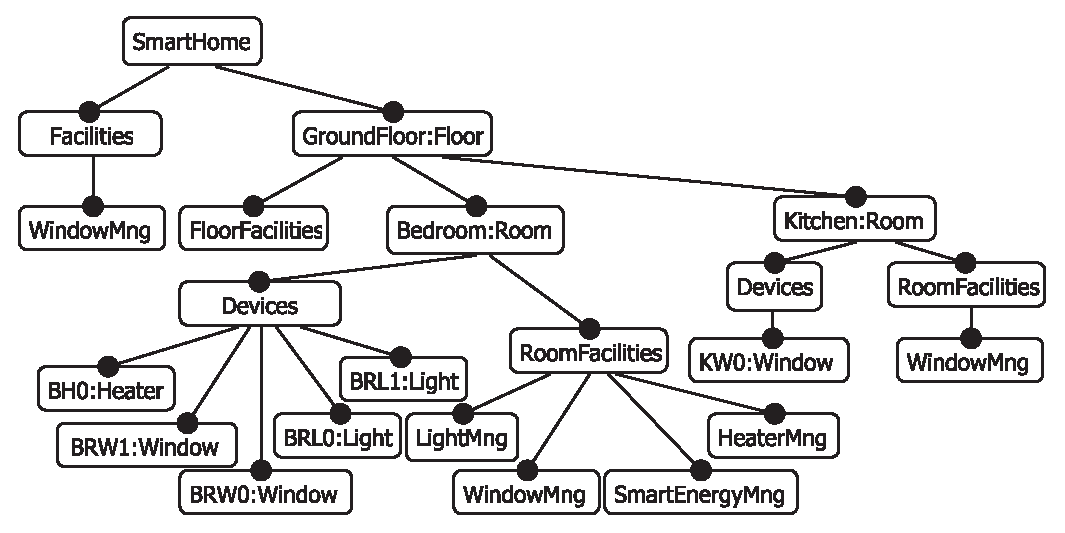
\includegraphics[width=\linewidth]{figures/configuration.eps} \\
  % 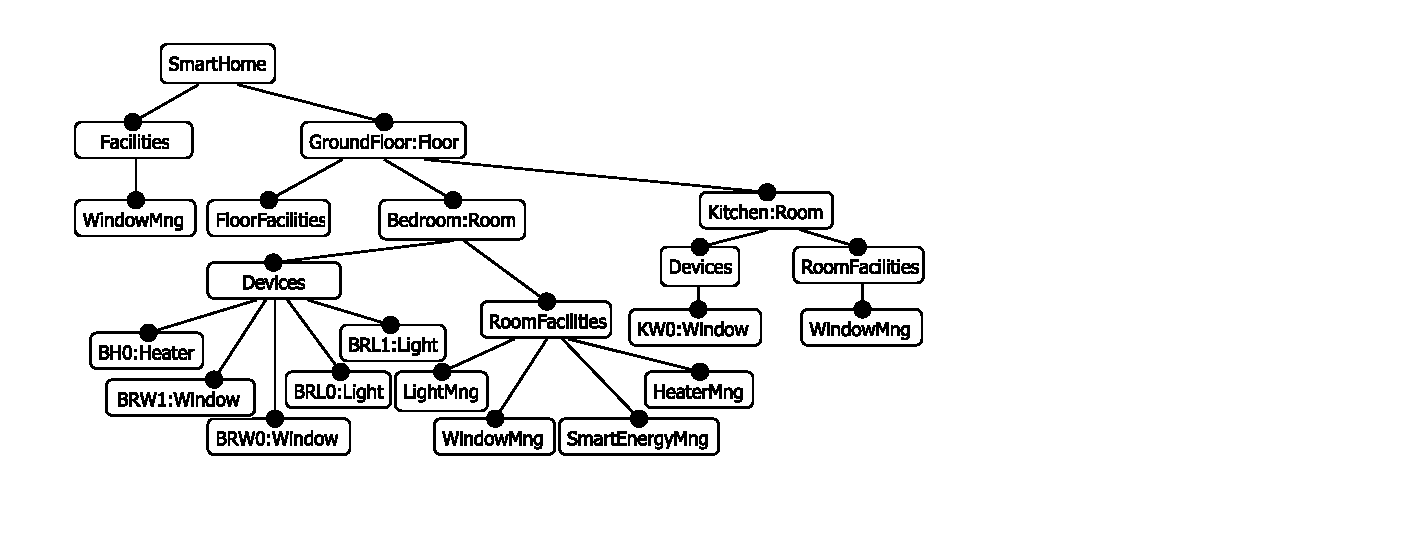
\includegraphics[width=\linewidth]{figures/configuration.pdf} \\
  \caption{Feature model for a SmartHome SPL}
  \label{fig:smartHomeCfg}
\end{figure}


The process of creating new feature instances is called \emph{cloning}~\cite{czarnecki:2005d,czarnecki:2005}. The semantics behind a cloning operation is that a new feature of the type of the clonable feature is created. Moreover, the subtree below the clonable feature is also cloned and copy below the newly created feature. This subtree can then be configured as any another feature model. To distinguish between different clones of a same feature, we have opted for giving to each clone a different name. Figure~\ref{fig:smartHomeCfg} shows a configuration of the feature model of Figure~\ref{fig:smartHomeFM}. It represents a really simple house, with only one floor and two rooms. It should be noticed that the subtree below \imp{Room} has been copied below the clones \imp{Kitchen} and \imp{Bedroom} and then configured, i.e. features have been selected, unselected or cloned.

It should be noticed that the usage of clonable features allows a more fine-grained configuration of software products. Due to the use of clones for the different floors and rooms, we can customize each floor and/or room individually. This would not be possible using traditional feature models, where we need to create separate feature models for each floor and room and be responsible for manually managing and synchronizing them, which can be a cumbersome and error prone tasks. Using feature models, these relationships are automatically secified and managed at the model level. For instance, all feature models related to rooms of a same floor are subtrees of a same parent, which is the clone for such a floor. For 
instance, all feature models related to rooms of a same floor are subtrees of a same parent, which is the clone for such 
a floor.

% , which would able to specify these facilities at the house, floor or room level. Therefore, to create a model similar to % the one depicted in Figure~\ref{fig:smartHomeFM}, we would have to create separate feature models for: (1) the whole 
% house; (2) each individual floor; and (3) each individual room. This might lead to scalability problems, as we would need 
% to manage a set of individual and unrelated feature models. Moreover, if some constraints, such as ``if \imp{HeaterMng} 
% is selected per house level, at least one \imp{Room} must contain a \imp{Heater}'', were defined, we would need to manage 
% different unrelated models at the same time in order to evaluate if this constraint is satisfied or not. This can be a 
% cumbersome and daunting task. Using clones, relationships between these different feature models are established. For 
% instance, all feature models related to rooms of a same floor are subtrees of a same parent, which is the clone for such % a floor. This help to simplify the problem of evaluating the previously described constraint.

% In this case, the process has been as follows: (1) we have create a clone for the \imp{Floor} feature; and we have called 
% it \imp{GroundFloor}. (2) We have removed the \imp{Floor} feature as more clones were not required; (3) Similarly, we 
% have created two clones of the \imp{Room} feature, one for the \imp{Kitchen} and other one for the {Bedroom}. The subtree 
% below Room was cloned and copied below the \imp{Kitchen} and \imp{Bedroom} features. (4) Then, we have created clones for 
% the devices which must be placed in each room according to the user requirements. (5) Finally, we have selected the \imp
% {WindowMng} facility for the entire house; all the facilities for the \imp{Bedroom}; and no extra facilities, beyond \imp
% {WindowMng}, for the \imp{Kitchen}. We have not defined any facility at the \imp{Floor} level.

This feature model makes also use of another advanced mechanisms for feature modelling, which are \emph{feature references}~\cite{czarnecki:2005}. A feature reference is a feature that references another feature. In Figure~\ref{fig:smartHomeFM}, \imp{FloorFacilities} and \imp{RoomFacilities} are feature references. Both them refer to \imp{Facilities} (this relationship is not explicitly displayed in the diagram). The semantics of a feature reference is to replace the feature reference with the subtree with root in the feature that is referenced. In our case, \imp{FloorFacilities} and \imp{RoomFacilities} would be replaced with the subtree with root in \imp{Facilities}. Feature references help to avoid redundancies in feature models, which contributes to scalability.


% It should be noticed that the used of clonable features allows a more fine-grained configuration of software products. 
% Due to the use of clones for the different floors and rooms, we can customize each floor and/or room individually. This 
% would not be possible using traditional feature models, which would able to specify these facilities at the house, floor 
% or room level. Therefore, to create a model similar to the one depicted in Figure~\ref{fig:smartHomeFM}, we would have 
% to create separate feature models for: (1) the whole house; (2) each individual floor; and (3) each individual room. This 
% might lead to scalability problems, as we would need to manage a set of individual and unrelated feature models. 
% Moreover, if some constraints, such as ``if \imp{HeaterMng} is selected per house level, at least one \imp{Room} must 
% contain a \imp{Heater}'', were defined, we would need to manage different unrelated models at the same time in order to 
% evaluate if this constraint is satisfied or not. This can be a cumbersome and daunting task. Using clones, relationships 
% between these different feature models are established. For instance, all feature models related to rooms of a same floor 
% are subtrees of a same parent, which is the clone for such a floor. This help to simplify the problem of evaluating the 
% previously described constraint.
